\documentclass[13pt, a4paper]{report}
\usepackage{xeCJK} %中文字體
\usepackage{hyperref} %引用url連結
\usepackage{listings} %引用程式碼
\usepackage{graphicx} %插入圖片
\usepackage{fontawesome5} %引用icon
\usepackage{amsfonts} %數學簍空的英文字
\usepackage{amsmath} %數學多行
\usepackage{indentfirst} %章節首段首行縮排
\usepackage{enumerate} %數字清單的編號
\usepackage[]{caption} %圖片標示
\usepackage{subfigure} %圖片並排
\lstset{language=Python, %設定語言
		basicstyle=\footnotesize, 
		frame=lines,
		caption={Python code}, %設定capion
		label={lst:example} %設定label
}
\graphicspath{{./Gradient descent optimizer/}} %圖片預設讀取路徑
\setCJKmainfont{SimSun} %設定中文字體
\linespread{1.5} %設定行距

\renewcommand\thepart{\arabic{part}}
\renewcommand{\figurename}{圖.} %設定圖片標示名稱
\renewcommand{\lstlistingname}{程式.} %設定程式標示名稱
\usepackage[margin=1.5cm]{geometry} %設定頁面邊緣
\title{神經網路梯度下降優化法}
\author{簡國龍}
\begin{document}
\maketitle
\tableofcontents

\chapter{Gradient Descent Optimizer}
\begin{figure}[hbt!]
\center
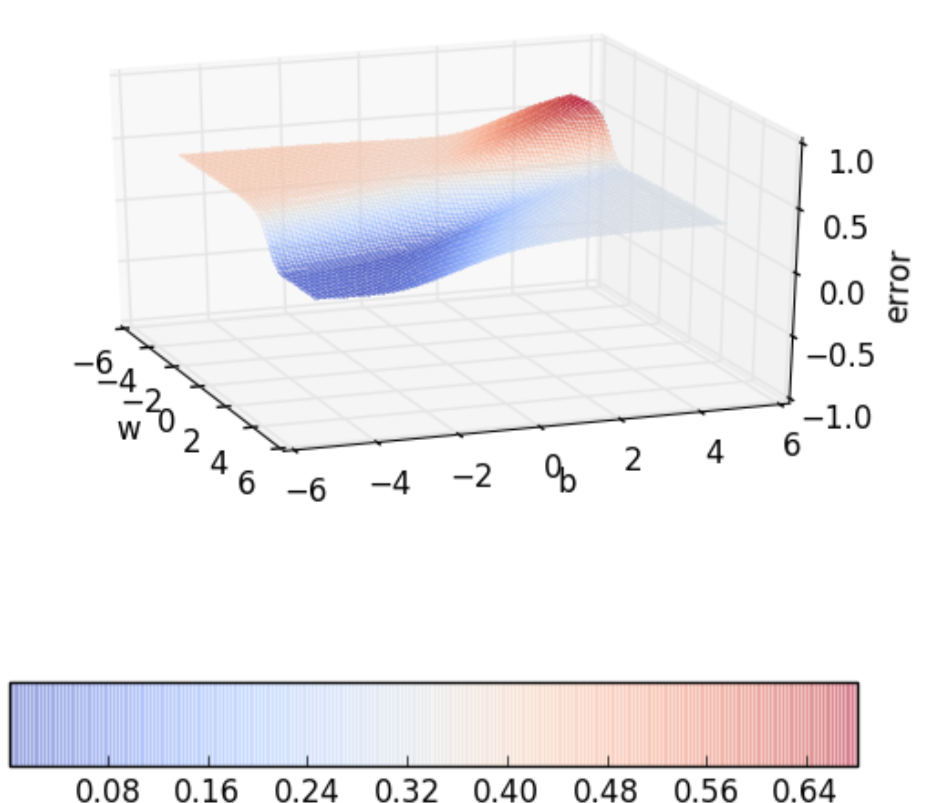
\includegraphics[width=8cm]{Error_surface}
\caption{Error surface \href{https://hackernoon.com/the-reason-behind-moving-in-the-direction-opposite-to-the-gradient-f9566b95370b}{\faLink}}\label{Fig.Error_surface} 
\end{figure}
Gradient descent (梯度下降)將目標函數$J_{(\theta)}$(下面是以loss function $L_{(\theta)}$當作目標函數)最小值化,藉由模型參數(model's parameters) $\theta \in \mathbb{R}^d$。\\
假設$\theta$是weight(w)和bias(b)的函數,是一個向量(matrix),隨機產生weight和bias的起始值
$$\overrightarrow{\theta_{(w, b)}}=(w, b)$$

假設$\overrightarrow{\Delta\theta}$是$\Delta w$(權重差值)和$\Delta b$(偏差差值)的函數,當loss值減少並落在error較小的地方,$\Delta\theta$就是在降低loss值,$\overrightarrow{\Delta\theta}$的向量參數就會像$\Delta\theta \in \mathbb{R}^d$,找到loss值最小的地方只需要$\theta$朝$\theta+\Delta\theta$方向移動就會找到。
$$\overrightarrow{\Delta\theta_{(w, b)}}=(\Delta w, \Delta b)$$

如果將$\overrightarrow{\Delta\theta}$和$\overrightarrow{\theta}$相加合成成$\overrightarrow{\theta_{R}}$(即[圖.\ref{Fig.theta_vector}]上的$\overrightarrow{\theta_{new}}$)。但要注意$\overrightarrow{\Delta\theta}$的值有可能過大就錯過廣域最小值的地方,所以係數$\eta$用來縮放$\overrightarrow{\Delta\theta}$的值,$\eta$是純量,通常是小於1(縮小)。因此
$$\overrightarrow{\theta_{R}}=\overrightarrow{\theta}+\eta\cdot\overrightarrow{\Delta\theta}$$

\begin{figure}[hbt!]
\center
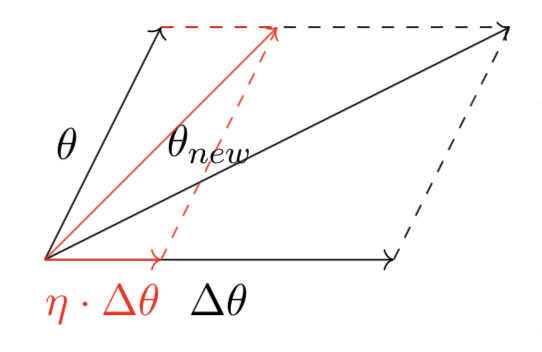
\includegraphics[width=8cm]{theta_vector}
\caption{theta vector \href{https://hackernoon.com/the-reason-behind-moving-in-the-direction-opposite-to-the-gradient-f9566b95370b}{\faLink}}
\label{Fig.theta_vector} 
\end{figure}

$\theta$剛開始是隨機產生的,但為了確保$\overrightarrow{\Delta\theta}$的方向是朝loss值減少的方向,所以要持續循環的計算才能達到廣域(絕對)最小值。為了找到正確的$\overrightarrow{\Delta\theta}$,所以將$\theta_{R}$以\href{https://youtu.be/3d6DsjIBzJ4}{\underline{泰勒級數}}方式表現,設$\overrightarrow{\Delta\theta}=u$
$$L_{(\theta+\eta u)}=L_{(\theta)}+\eta u^{T}\cdot\bigtriangledown_{\theta} L_{(\theta)}+\frac{\eta^2}{2!}u^T\cdot\bigtriangledown^2 L_{(\theta)}u+\frac{\eta^3}{3!}...+\frac{\eta^4}{4!}...+\frac{\eta^n}{n!}...$$


從泰勒級數中得知$\theta$在特定值並做很小的更動,loss function($L_{(\theta)}$)就會產生新的值,大幅減少每次更動$\theta$所計算廣域最小值的次數(若不是以泰勒級數的型式描述,當每次更動$\theta$就必需跌代出廣域最小值;泰勒級數的型式則會隨$\theta$些微的更動產生新值)
$$\bigtriangledown L_{(\theta)}=[\frac{\partial L_{(\theta)}}{\partial w}, \frac{\partial L_{(\theta)}}{\partial b}]$$


$\eta$值通常小於一,當$\eta ^2<<1$,因此可以忽略高階項(若要求更高的精度可不忽略)
$$L_{(\theta+\eta u)}=L_{(\theta)}+\eta u^{T}\cdot\bigtriangledown_{\theta} L_{(\theta)} [\eta\ is\ typically\ small, so\ \eta^2, \eta^3,\cdots \rightarrow 0]$$
新的$L(\theta+\eta u)$輸出的值會小於$L_{(\theta)}$
$$L_{(\theta+\eta u)}-L_{(\theta)}<0$$
同理可證
$$u^{T}\cdot\bigtriangledown_{\theta} L_{(\theta)}<0$$
符合這條件$u$ :當新的值小於舊的值,$u$就是一個好的值。
假設$\overrightarrow{u}$和$\overrightarrow{\bigtriangledown_{\theta} L_{(\theta)}}$的夾角為$\beta$ \href{https://www.khanacademy.org/math/linear-algebra/vectors-and-spaces/dot-cross-products/v/vector-dot-product-and-vector-length}{\faLink}
$$\cos(\beta)=\frac{u^{T}\cdot\bigtriangledown_{\theta} L_{(\theta)}}{\vert u^{T}\vert\vert \bigtriangledown_{\theta} L_{(\theta)}\vert}$$
因為$\cos_{(\theta)}$的值介於1和-1之間
$$-1<\cos(\beta)=\frac{u^{T}\cdot\bigtriangledown_{\theta} L_{(\theta)}}{\vert u^{T}\vert\vert \bigtriangledown_{\theta} L_{(\theta)}\vert}\leq 1$$

$$assume\ k=\vert u^{T}\vert\vert \bigtriangledown_{\theta} L_{(\theta)}\vert \ the\  inequalities\ simplify\ to$$
$$-k \leq k\cos(\beta)=u^{T}\cdot\bigtriangledown_{\theta} L_{(\theta)}\leq k$$
所以盡可能的讓新值小於舊值($L_{(\theta+\eta u)}-L_{(\theta)}<0$),loss值就會減少得越多。因此$u^{T}\cdot\bigtriangledown_{\theta} L_{(\theta)}$應該盡可能為負,在這情況下$\cos(\beta)$應該等於$-1$,$\beta$的角度為$180^{\circ} $,這就是與梯度方向相反的原因。

梯度下降法告訴我們:當$\theta$在特定值,並想減少新的$\theta$值,使loss值逐漸減少就應該與梯度相反的方向找(梯度為正值,找最小值就需往負的方向找)
$$w_{t=1}=w_t-\eta\bigtriangledown w_t$$
$$b_{t=1}=b_t-\eta\bigtriangledown b_t$$
$$where\ at\ w=w_t,b=b_t$$
$$
	\begin{cases}
	\bigtriangledown w_t=\frac{\partial L_{_{(\theta)}}}{\partial w}\\
	\bigtriangledown b_t=\frac{\partial L_{_{(\theta)}}}{\partial b}
	\end{cases}
$$
\newpage
\chapter{\href{https://ruder.io/optimizing-gradient-descent/}{Stochastic gradient descent}}
\section{Batch gradient descent}
Vanilla gradient descent又稱Batch gradient descent(批次梯度下降法),計算成本函數的梯度,參數$\theta$對於整個訓練資料:
$$\theta=\theta-\eta\cdot\bigtriangledown_{\theta}L_{(\theta)}$$

成本函數可以當作loss function,因此直接以$L_{(\theta)}$表示,參數$\theta$為weight和bias的函數,$\eta$為學習率。由於計算整個資料集計算梯度只更新一次,Bath gradient descent可能非常慢並且對於資料集無法符合及記憶體來說棘手(一次需要儲存整個資料集的資料,當更新和計算時會占用大量記憶體)。他也無法使用在在線更新模型,就是無法即時有新的範例。Bath gradient descent寫成程式碼[程式.\ref{code.Batch gradient descent}]就會像這樣:

\begin{center}
\begin{lstlisting}[caption=Batch gradient descent]
for i in range(nb_epochs):
  params_grad = evaluate_gradient(loss_function, data, params)
  params = params - learning_rate * params_grad
\end{lstlisting}
\label{code.Batch gradient descent}
\end{center}

預定義每次epoch,先計算loss function梯度向量對於整個資料集參數向量。最先進的深度學習資料庫備自動區別功能,對於一些參數有效地計算梯度。如果梯度值來自於先前計算出的梯度值,那檢查就會梯度,並以梯度相反的方向更新參數,學習率決定多大的更新量。Batch gradient descent對於凸面誤差可以保證收斂到廣域最小值,對於非面凸誤差可以收斂到局部最小值。
\section{Stochastic gradient descent}
Stochastic gradient descent(SGD)隨機梯度下降法,這裡的目標函數為$J_{(\theta,x^i,y^i)}$(變數$\theta$為w(weight)和b(bias)的函數,也可以寫成$J_{(w, b, x^i, y^i)}$)。
$$\theta=\theta-\eta\cdot\bigtriangledown_{\theta}J_{(\theta, x^i, y^i)}$$
批量梯度下降他會在每個參數更新前重新計算相似梯度。SGD每次次執行會更新來消除多餘(誤差),因此通常速度很快,也可用於在線學習。SGD頻繁更新並變化很大,因為目標方程式波動很大[圖.\ref{Fig.SGD_fluctuation}]。SGD的方程式一方面會跳到新的值和潛在局部最小值,另一方面SGD會持續超調(誤差超過預期)最後收斂到廣域最小值。

無論如何他被顯示當學習率下降緩慢,SGD顯示與Batch gradient descent同樣收斂行為,幾乎可以肯定地,對於凸面或非凸面優化,會收斂到絕對或是局部最小值。
\newpage
這程式碼片段[程式.\ref{code.Stochastic gradient descent}]在訓練樣本上加入一個迴圈來對每個樣本評估梯度。每個epoch(訓練循環)會打亂訓練數據。
\begin{center}
\begin{lstlisting}[caption=Stochastic gradient descent]
for i in range(nb_epochs):
  np.random.shuffle(data)
  for example in data:
    params_grad = evaluate_gradient(loss_function, example, params)
    params = params - learning_rate * params_grad
\end{lstlisting}
\label{code.Stochastic gradient descent}
\end{center}
\begin{figure}[hbt!]
\center
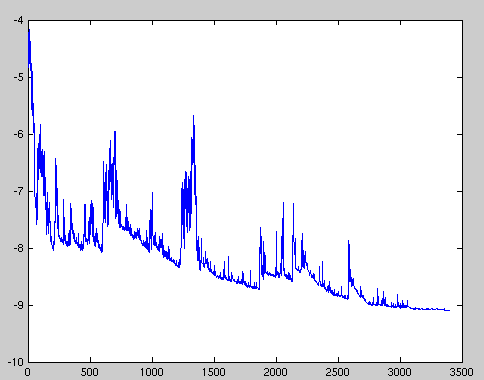
\includegraphics[width=8cm]{sgd_fluctuation}
\caption{SGD fluctuation \href{https://ruder.io/optimizing-gradient-descent/}{\faLink}} 
\label{Fig.SGD_fluctuation}
\end{figure}
\section{Mini-batch gradient descent}
Mini-batch gradient descent(小批量梯度下降)各取前兩者的優點,將資料集分割成小區塊,每個小區塊大小稱作batch size,每次跑完batch size算迭代(iteration)一次,算完一次資料集即完成一次epoch。舉例:資料集大小為1000,若batch size為50,iteration為$\frac{datasets}{batch\_size}=\frac{1000}{50}=20$,當iteration跑完20次算完成一次epoch。

這方式可以減少參數更新的方差,並且可以穩定收斂;可利用最先進的深度學習庫所共有的高度優化的矩陣優化,從而由一個小批量計算出梯度非常有效。通常batch sizes的範圍介於50 \textasciitilde 256,會因為應用而有所差異。訓練神經網絡時,通常選擇Mini-batch gradient descent算法,而當使用這算法時,通常也使用術語SGD。
$$\theta=\theta-\eta\cdot\bigtriangledown_{\theta}J_{(\theta, x^{(i:i+n)}, y^{(i:i+n)})}$$
下面程式碼[程式.\ref{code.Mini-batch gradient descent}]為迭代範例,batch size大小為50:
\begin{center}
\begin{lstlisting}[caption=Mini-batch gradient descent]
for i in range(nb_epochs):
  np.random.shuffle(data)
  for batch in get_batches(data, batch_size=50):
    params_grad = evaluate_gradient(loss_function, batch, params)
    params = params - learning_rate * params_grad
\end{lstlisting}
\label{code.Mini-batch gradient descent}
\end{center}
\section{Challenges}
Mini-batch gradient descent無論如何還是無法確保收斂的很好,存在一些需要解決的挑戰:
\begin{enumerate}
\item 選擇適當的學習率是有難度的。如果學習率太小會導致收斂困難或緩慢,學習率太大則會阻礙收斂導致loss function來回波動或發生偏離。
\item 學習率清單嘗試在訓練的時候調整學習率,即根據預定義清單或當目標下降於閾值(threshold)時降低學習率。但清單和閾值須預先定義,因此無法適應數據集的特徵。
\item 另外相同學習率適用全部參數更新。如果資料稀疏而且外型有很特別的頻率,我們可能不希望將所有特徵更新到相同的程度,而是對很少發生的特徵執行較大的更新。
\item 最小化神經網路常見的高度非凸面誤差方程式(error function)的另一關鍵挑戰則是要避免被困在大量次優的局部最小值區域中。認為困難實際上不是由局部最小值引起的,而是由鞍點引起的,即一維向上傾斜而另一維向下傾斜的點。這些鞍點通常被相同誤差的平穩段包圍,這使得SGD很難逃脫,因為在所有維度上梯度都接近於零。
\newcounter{enumii_saved}
\setcounter{enumii_saved}{\value{enumii}}
\end{enumerate}

\chapter{Gradient descent optimization algorithms}
在下文中,整理概述深度學習社區廣泛使用的一些算法來應對上述挑戰。我們不會討論在實際中無法計算高維數據集的算法,例如二階法、牛頓法。
\section{Momentum}
SGD難以在陡峭的往正確的方向,那就是說在一個維度上,曲面的彎曲比另一個維度要陡得多,這在局部最優情況下很常見。在這些情況下,SGD會在陡峭的地方振盪,而僅沿著底部朝著局部最優方向猶豫前進,如[圖.\ref{Fig.SGD_without_momentum}]所示。

Momentun(動量)是一個幫助加速SGD在正確方向和抑制震盪的方法,在[圖.\ref{Fig.SGD_with_momentum}]。
\begin{figure}[htbp]
\centering
\subfigure[SGD without momentum]{
\begin{minipage}[t]{0.25\linewidth}
\centering
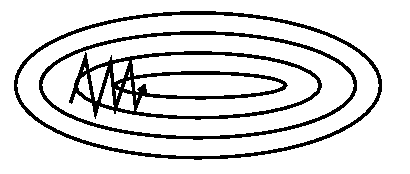
\includegraphics[width=1in]{without_momentum}
\label{Fig.SGD_without_momentum}
\end{minipage}}
\subfigure[SGD with momentum]{
\begin{minipage}[t]{0.25\linewidth}
\centering
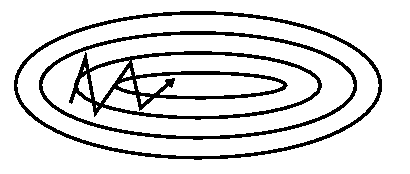
\includegraphics[width=1in]{with_momentum}
\label{Fig.SGD_with_momentum}
\end{minipage}}

\centering
\caption{SGD momentum}
\end{figure}

這麼做會增加一個係數$\gamma$來更新上次的向量到正確向量(修正偏差),$\gamma$通常設為0.9左右。
$$v_t = \gamma v_{t-1}+\eta\cdot\bigtriangledown_{\theta}J_{(\theta)}$$
$$\theta = \theta-v_t$$

實際上,使用動量的時候,就像將球推下山坡。球在下坡時滾動時會累積動量,在途中速度會越來越快(如果存在空氣阻力,直到達到極限速度,也就是$\gamma <1$)參數更新也發生了同樣的事情:動量(momentum )對於梯度指向相同方向的維度增加,而對於梯度改變方向的維減少動量。結果,我們獲得了更快的收斂並減少了振盪。
\section{Nesterov accelerated gradient}
然而,Momentun的做法就像,一個球從山上滾下來,盲目地跟隨斜坡。我們希望有一個更聰明的球,這個球有一個去向的概念,以便在山坡再次變高之前知道它會減速。

Nesterov accelerated gradient(NAG)是一種使動量具有這種先見之明的方式。我們知道使用動量$\gamma v_{t-1}$來移動參數θ。計算$\theta - \gamma v_{t-1}$這樣就給了參數的下一個位置的近似值(完整更新缺少的梯度),這是參數將要存在的大致概念。現在,通過計算與當前參數無關的梯度來有效地看到目前的參數$\theta$將會移動到的位置:
$$v_t = \gamma v_{t-1}+\eta\cdot\bigtriangledown_{\theta}J_{(\theta-\gamma v_{t-1})}$$
$$\theta = \theta - v_t$$

同樣,我們設置動量$\gamma$約為0.9。動量首先計算當前梯度([圖.\ref{Fig.NAG}]中的藍色小向量),然後在更新的累積梯度(藍色向量)的方向上發生較大的跳躍,而NAG首先在先前的累積梯度的方向上進行較大的跳躍(棕色向量),測量梯度,然後進行校正(紅色向量),從而完成NAG更新(綠色向量)。這種預期的更新可防止我們過快地進行,並導致響應速度增加,從而顯著提高了RNN在許多任務上的性能。有關NAG背後另一解釋,\href{https://cs231n.github.io/neural-networks-3/}{\underline{請參見此處}},而Ilya Sutskever在其博士論文中給出了更詳細的概述。
\begin{figure}[hbt!]
\center
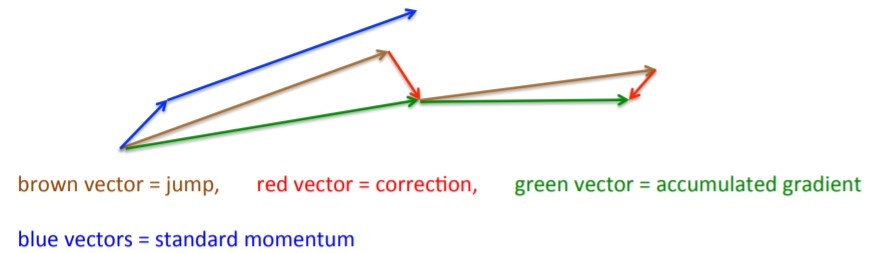
\includegraphics[width=15cm]{NAG}
\caption{NAG \href{http://www.cs.toronto.edu/~tijmen/csc321/slides/lecture_slides_lec6.pdf}{\faLink}} 
\label{Fig.NAG}
\end{figure}

既然能夠使更新適應誤差函數的斜率並依次提高SGD,我們還希望使更新適應每個單獨的參數,以根據其重要性執行更大或更小的更新。
\section{Adagrad}
Adagrad是一個梯度優化的算法,它可以做到:學習率適應參數,對於頻繁出現的特徵相關參數執行較小的更新(較低的學習率),以及對不經常出現的特徵相關參數進行較大更新(即學習率較高)。Adagrad可以提高SGD的強度,用於訓練大型神經網絡。

先前,在同一次$\theta$參數(更新後就算另一次),每個$\theta$都使用相同的$\eta$(學習率)。Adagrad則是對每個$\theta$參數使用不同的$\eta$,t代表time step。先將Adagrad的參數更新向量化。用$g_t$表示time step的梯度,$g_{t,i}$表示目標函數(參數$\theta$在time step $t$)對參數做偏微分計算。
$$g_{t,i}=\bigtriangledown_{\theta}J_{(\theta_{t,i})}$$

當SGD更新每個參數$\theta_i$,在每個time step $t$,因此變成:
$$\theta_{t+1,i}=\theta_{t,i}-\eta\cdot g_{t,i}$$

更新規則,Adagrad根據先前$\theta_i$計算的梯度,對每個參數$\theta_i$修改整個學習率$\eta$在每個time step$t$:
$$\theta_{t+1,i}=\theta_{t,i}-\frac{\eta}{\sqrt{G_{t,ii}+\epsilon}}$$

$G_t \in \mathbb{R}^{d\times d}$這是一個對角矩陣每個對角元素$i$,$i$是關於$\theta$梯度平方和取決於time step$t$,$\epsilon$是避免分母為0($\epsilon$通常為$1\times10^{-8}$),如果沒有平方根運算,該算法的性能將大大降低。

$G_t$包含了過去梯度平方根,由於全部$\theta$參數沿著對角線,通過向量的內積計算$G_t$和$g_t$:
$$\theta_{t+1}=\theta_{t}-\frac{\eta}{\sqrt{G_{t}+\epsilon}}\cdot g_t$$

Adagrad主要好處之一是,無需手動調整學習率。大多數實現使用預設值0.01並將其保留為預設值。Adagrad主要弱點是會累積分母的平方梯度:由於每項都是正的,累積和會在訓練中不斷增長。反過來,學習率下降,並最終變得無限小,這算法就不再獲得知識。
\section{Adadelta}
Adadelta是Adagrad的延伸,下降其激進的程度,單調的降低學習率。Adadelta會限制過去累積的梯度,並將其限制在某個特定大小$w$,並代替Adagrad過去累積的梯度平方。不是低效的存儲$w$先前的平方梯度,而是梯度總和是遞迴定義為所有過去衰減梯度平方平均值。流動平均$E[g^2]_t$在time step $t$然後取決於(像Momentum的$\gamma$)先前平均和最近梯度:
$$E[g^2]_t=\gamma E[g^2]_{t-1}+(1-\gamma)g^2 _t$$

$\gamma$值和Momentum的相似,約為0.9,現在根據參數更新向量$\bigtriangleup\theta_t$來重寫SGD:
$$\bigtriangleup\theta_t=-\eta\cdot g_{t,i}$$
$$\theta_{t+1}=\theta_t+\bigtriangleup\theta_t$$

Adagrad的參數更新向量替換成:對角矩陣$G_t$過去梯度平方的衰退平均$E[g^2]_t$
$$\bigtriangleup\theta_t=-\frac{\eta}{\sqrt{G_t+\epsilon}}\cdot g_t$$
$$replace\ G_t\ with\ E[g^2]_t\Rightarrow\bigtriangleup\theta_t=-\frac{\eta}{\sqrt{E[g^2]_t+\epsilon}}\cdot g_t$$

由於分母只是梯度的均方根(RMS),我們可以取代成縮寫:
$$\bigtriangleup\theta_t=-\frac{\eta}{RMS[g]_t}\cdot g_t$$

這個更新單位和SGD、Momentum以及Adagrad的單位不符合,因此更新需有相同的參數。為了實現這一點,首先定義另一個指數衰減平均值,這次不是梯度平方更新而是參數平方更新:
$$E[\bigtriangleup\theta^2]_t=\gamma E[\bigtriangleup\theta^2]_{t-1}+(1-\gamma)\bigtriangleup\theta^2 _t$$

RMS參數更新:
$$RMS[\bigtriangleup\theta]_t=\sqrt{E[\bigtriangleup\theta^2]_t+\epsilon}$$

$RMS[\bigtriangleup\theta]_t$是未知的,更新參數的RMS取近似直到上個time step。用$RMS[\bigtriangleup\theta]_{t-1}$取代學習率$\eta$,最後產生新的規則:
$$\bigtriangleup\theta_t=-\frac{RMS[\bigtriangleup\theta]_{t-1}}{RMS[g]_t}g_t$$
$$\theta_{t+1}=\theta_t+\bigtriangleup\theta_t$$

使用Adadelta,甚至不需要設定預設學習率,因為它已從更新規則淘汰。
\section{RMSprop}
RMSprop是Geoffrey Hinton在\href{http://www.cs.toronto.edu/~tijmen/csc321/slides/lecture_slides_lec6.pdf}{他的課程}中提出的未公開自適應學習率的方法。

RMSprop和Adadelta都是為了解決Adagrad的學習率急劇下降的問題個別獨立開發出來的解決方式。RMSprop實際上與Adadelta得出的第一個更新向量相同:
$$E[g^2]_t=0.9E[g^2]_t+0.1g^2 _t$$
$$\theta_{t+1}=\theta_t-\frac{\eta}{\sqrt{E[g^2]_t+\epsilon}}g_t$$

RMSprop也將學習率除以梯度平方的指數衰減平均值。Hinton建議$\gamma$設為0.9,好的預設學習率$\eta$數值為0.001。
\section{Adam}
Adaptive Moment Estimation自適應矩評估(Adam) 是另一種計算每個評估學習率的方法。出了儲存過去梯度平方的指數衰減平均值$v_t$,就像Adadelta和RMSprop一樣,Adam還保留過去梯度的指數衰減平均值$m_t$,類似動量(Momentum)。如果Momentum被視為順著斜坡下滑的球,而Adam則是像一個帶有摩擦的沉重的球,因此更適合待在error face平坦的最小值區域。計算過去梯度平方的衰減平均值$m_t$和$v_t$分別如下:
$$m_t=\beta_1 m_{t-1}+(1-\beta_1)g_t$$
$$v_t=\beta_2 v_{t-1}+(1-\beta_2)g^2 _t$$

$m_t$和$v_t$分別是第一階矩平均估計值和第二階矩無中心方差估計值,因此是方法的名稱。像$m_t$和$v_t$被初始化為向量$o$,Adam的作者觀察到它們偏向零,特別是在初始time step,尤其是在衰減率較小的時候(也就是說$\beta_1$和$\beta_2$趨近於1)藉由計算校正偏差第一矩和第二矩抵消偏差:
$$\hat{m}_t = \dfrac{m_t}{1 - \beta^t_1} $$ 
$$\hat{v}_t = \dfrac{v_t}{1 - \beta^t_2} $$

使用他們去更新參數,就像Adadelta和RMSprop中所看到的那樣,這將產生Adam更新規則:
$$\theta_{t+1} = \theta_{t} - \dfrac{\eta}{\sqrt{\hat{v}_t} + \epsilon} \hat{m}_t$$

$\beta_1$預設值建議為0.9,$\beta_2$預設值建議為0.999,$\epsilon$預設值建議為$10^{-8}$。根據經驗證明Adam表現良好,並且與其他自適應學習算法相比具有優勢。
\section{AdaMax}
在Adam更新規則中的$v_t$係數是與梯度成反比地縮放過去梯度的範數(通過$v_{t-1}$項)和當前梯度$|g_t|^2$:
$$v_t = \beta_2 v_{t-1} + (1 - \beta_2) |g_t|^2$$
我們轉換這個更新到$\ell_p$。注意$\beta_2$參數化為$\beta_2^p$:
$$v_t = \beta_2^p v_{t-1} + (1 - \beta_2^p) |g_t|^p$$

大規範$p$值使數值上變得不穩定,這就是為什麼$\ell_1$和$\ell_2$規範在實踐中是最常見的。然而,$\ell_\infty$通常也表現出穩定的行為。作者(Kingma and Ba, 2015)提出了AdaMax並證明了和$\ell_\infty$收斂到更穩定的值。為了避免與Adam混用,所以使用$u_t$來表示無窮範數約束$v_t$:
$$u_t = \beta_2^\infty v_{t-1} + (1 - \beta_2^\infty) |g_t|^\infty$$
$$ = \max(\beta_2 \cdot v_{t-1}, |g_t|) $$

替換為Adam更新公式$\sqrt{\hat{v}_t} + \epsilon$和$u_t$得出AdaMax更新規則:
$$\theta_{t+1} = \theta_{t} - \dfrac{\eta}{u_t} \hat{m}_t$$

注意$u_t$依靠最大運算,不建議Adam中的$m_t$和$v_t$偏向零,這就是為什麼不需要針對$u_t$計算偏差。好的預設值$\eta=0.002$,$\beta_1=0.9$和$\beta_2=0.999$。
\section{Nadam}
Adam可以看作是RMSprop和的組合:RMSprop貢獻了過去梯度平方的指數衰減平均值$v_t$,而Momentum則代表過去梯度指數的衰減平均值。還看到Nesterov accelerated gradient (NAG) 優於Vanilla momentum。

Nadam (Nesterov-accelerated Adaptive Moment Estimation,Nesterov加速的自適應矩估計),因此結合了Adam和NAG。為了將NAG納入Adam,需要修改動量項$m_t$。使用先前符號回顧動量更新規則:
$$g_t = \nabla_{\theta_t}J(\theta_t)$$
$$m_t = \gamma m_{t-1} + \eta g_t$$
$$\theta_{t+1} = \theta_t - m_t $$

$J$是目標函數,$\gamma$是動量衰減項,$\eta$是step size(學習率),上面的第三個方程式擴展為:
$$\theta_{t+1} = \theta_t - ( \gamma m_{t-1} + \eta g_t)$$

再次證明了動量涉及在前一個動量向量的方向上往前一步和在當前梯度的方向上邁出一步。NAG然後允許計算梯度之前透過更新動量步長參數使梯度方向上執行更精確的步長。因此,我們只需要修改梯度$g_t$到達NAG:
$$g_t = \nabla_{\theta_t}J(\theta_t - \gamma m_{t-1})$$ 
$$m_t = \gamma m_{t-1} + \eta g_t$$
$$\theta_{t+1} = \theta_t - m_t$$

Dozat建議以以下方式修改NAG:一次用於更新梯度$g_t$第二次更新參數$\theta_{t+1}$,而不是應用momentum step兩次,現在直接應用前瞻動量向量來更新當前參數:
$$g_t = \nabla_{\theta_t}J(\theta_t)$$
$$m_t = \gamma m_{t-1} + \eta g_t$$
$$\theta_{t+1} = \theta_t - (\gamma m_t + \eta g_t)$$

為了將Nesterov動量添加到Adam,可以類似地用當前動量向量替換以前的動量向量。回想一下Adam更新規則如下:
$$m_t = \beta_1 m_{t-1} + (1 - \beta_1) g_t$$
$$\hat{m}_t = \frac{m_t}{1 - \beta^t_1}$$
$$\theta_{t+1} = \theta_{t} - \frac{\eta}{\sqrt{\hat{v}_t} + \epsilon} \hat{m}_t $$

用定義拓展第二個方程式:
$$\theta_{t+1} = \theta_{t} - \frac{\eta}{\sqrt{\hat{v}_t} + \epsilon} (\frac{\beta_1 m_{t-1}}{1 - \beta^t_1} + \frac{(1 - \beta_1) g_t}{1 - \beta^t_1})$$

注意$\frac{\beta_1 m_{t-1}}{1 - \beta^t_1}$只是前一個的time step的動量向量的偏差來校正評估。因此,可以將其替換為$\hat{m}_{t-1}$:
$$\theta_{t+1} = \theta_{t} - \frac{\eta}{\sqrt{\hat{v}_t} + \epsilon} (\beta_1 \hat{m}_{t-1} + \frac{(1 - \beta_1) g_t}{1 - \beta^t_1})$$

為簡化,因為無論如何將在下一步中替換分母,所以忽略了分母$1 - \beta^t_1$。該方程式再次看起來和上面擴展的動量更新規則非常相似。可以像以前一樣添加Nesterov動量,方法是用當前動量向量偏差校正後的評估值替換前一時間步長的動量向量偏差校正後的評估值,這為我們提供了Nadam更新規則:
$$\theta_{t+1} = \theta_{t} - \frac{\eta}{\sqrt{\hat{v}_t} + \epsilon} (\beta_1 \hat{m}_t + \frac{(1 - \beta_1) g_t}{1 - \beta^t_1})$$
\section{AMSGrad}
\href{https://ruder.io/optimizing-gradient-descent/index.html#fn19}{\underline{Reddi等}}(2018)。正式化了這個問題,並指出了泛化行為不佳的原因:將過去梯度平方的指數移動平均值作為自適應學習率方法。雖然引入指數平均值的動機很充分:應防止學習率隨著訓練的進行而變得無限小;但這也是Adagrad算法的關鍵缺陷。在其他情況下,短期記憶的梯度成為障礙。

在Adam收斂到次優解的環境中,已經觀察到一些小型批次提供了較大且信息豐富的梯度,但是由於這些小型批次很少出現,因此指數平均會減小其影響,從而導致收斂性較差。作者(資料來源的作者)提供了一個簡單的凸型優化問題的例子,其中Adam可以觀察到相同的行為。

為了解決此問題,作者提出了一種新算法AMSGrad,該算法使用了過去梯度平方的最大值$v_t$而不是指數平均值來更新參數。$v_t$的定義與先前的Adam相同:
$$v_t = \beta_2 v_{t-1} + (1 - \beta_2) g_t^2$$

而不是直接使用$v_t$(或其偏差更正的版本$\hat{v}_t$),如果現在使用以前值的大於現在的值:
$$\hat{v}_t = \text{max}(\hat{v}_{t-1}, v_t)$$

這方式AMSGrad的不會增加步長(step size),從而避免了Adam遇到的問題。為了簡化,AMSGrad去除了Adam的去偏差(debias)步驟。可以看到完整的AMSGrad更新,沒有經過偏差校正的估計:
$$m_t = \beta_1 m_{t-1} + (1 - \beta_1) g_t $$ 
$$v_t = \beta_2 v_{t-1} + (1 - \beta_2) g_t^2$$ 
$$\hat{v}_t = \text{max}(\hat{v}_{t-1}, v_t)$$ 
$$\theta_{t+1} = \theta_{t} - \frac{\eta}{\sqrt{\hat{v}_t} + \epsilon} m_t$$

在小型數據集和CIFAR-10上,與Adam相比,性能有所提高。但是,其他實驗顯示其性能與Adam相似或更差。在實際運用,AMSGrad是否能勝過Adam,還有待觀察。有關深度學習優化的最新進展的更多信息,請參閱此\href{https://ruder.io/deep-learning-optimization-2017/}{\underline{blog文章}}。
\section{Gradient noise} 
增加noise跟隨高斯分布$N(0, \sigma^2_t)$ 對每個梯度更新:
$$g_{t, i} = g_{t, i} + N(0, \sigma^2_t)$$

根據排定時間對差異計算:
$$\sigma^2_t = \frac{\eta}{(1 + t)^\gamma}$$
添加這種noise 對不良初始化的網絡可使其更強化,並有助於訓練特別深且復雜的網絡。他們懷疑增加的噪聲使模型有更多的機會逃脫並找到新的局部極小值,這對於更深的模型而言更常見。
\section{其他最近的優化器}
在AMSGrad之後,已經提出了許多其他優化器。其中包括AdamW ,可以修復Adam的權重下降;QHAdam,將標準SGD步長與動量SGD步長進行平均;和AggMo,它結合了多個動量項$\gamma$和別的。有關最近的梯度下降算法的概述,請參閱此\href{https://johnchenresearch.github.io/demon/}{\underline{blog文章}}。











\end{document}
